\documentclass[a4paper,12pt,bold,leqno,fleqn,]{scrartcl}

\renewcommand{\baselinestretch}{1.3}\normalsize	

\renewcommand{\arraystretch}{1.2}
\newcommand{\vect}[1]{\mathbf{#1}}
\newcommand{\thin}{\thinspace}
\newcommand{\thick}{\thickspace}

\newcommand{\N}{\mathrm{N}}	%Normal Distribution
\newcommand{\U}{\mathrm{U}}	%Uniform Distribution
\newcommand{\D}{\mathrm{D}}	%Dirichlet Distribution
\newcommand{\W}{\mathrm{W}}	%Wishart Distribution
\newcommand{\E}{\mbox{E}}		%Expectation
\newcommand{\Iden}{\mathbb{I}}	%Identity Matrix
\newcommand{\Ind}{\mathrm{I}}	%Indicator Function

\newcommand{\var}{\mathrm{var}\thin}
\newcommand{\plim}{\mathrm{plim}\thin}
\newcommand{\cov}{\mathrm{cov}\thin}
\newcommand\indep{\protect\mathpalette{\protect\independenT}{\perp}}
\def\independenT#1#2{\mathrel{\rlap{$#1#2$}\mkern5mu{#1#2}}}

\usepackage{multicol}
\usepackage[sans]{dsfont}
\usepackage[round,longnamesfirst]{natbib}
\usepackage{bm}																									%matrix symbol
\usepackage{setspace}																						%Fu�noten (allgm. 
\usepackage{hyperref}
%Zeilenabst�nde)
\usepackage{threeparttable}
\usepackage{lscape}																							%Querformat
\usepackage[latin1]{inputenc}																		%Umlaute
\usepackage{graphicx}
\usepackage{amsmath}
\usepackage{amssymb}
\usepackage{fancybox}																						%Boxen und Rahmen
\usepackage{appendix}
\usepackage{enumerate}
\usepackage{tabularx}	
\usepackage[labelfont=bf]{caption}
\usepackage{longtable}																					%Mehrseitige Tabellen
\usepackage{color,colortbl}																			%Farbige Tabellen
\usepackage[left=2cm, right=2cm, top=2cm, bottom=3cm]{geometry} %Seitenr�nder
%\usepackage[normal]{caption2}[2002/08/03]												%Titel ohne float - Umgebung	
\definecolor{lightgrey}{gray}{0.95}	%Farben mischen
\definecolor{grey}{gray}{0.85}
\definecolor{darkgrey}{gray}{0.80}

\newcommand{\mc}{\multicolumn}
\parindent0pt

\newtheorem{Definition}{Definition}
\newtheorem{Remark}{Remark}
\newtheorem{Lemma}{Lemma}
\newtheorem{Theorem}{Theorem}
\newtheorem{Excercise}{Excercise}
\newtheorem{Result}{Result}
\newtheorem{Proposition}{Proposition}
\newtheorem{Prediction}{Prediction}
\newtheorem{Solution}{Solution}
\newtheorem{Problem}{Problem}

\setlength{\skip\footins}{1.0cm}			
\deffootnote[1em]{1.1em}{0em}{\textsuperscript{\thefootnotemark}}						
\renewcommand{\arraystretch}{1.05}

\usepackage{listings}
\usepackage{enumitem}
\newcommand{\inlineterminal}[1]{\colorbox{black}{\lstinline[basicstyle=\ttfamily\color{white}]|#1|}}
\makeatletter
\newenvironment{manquotation}[2][2em]
  {\setlength{\@tempdima}{#1}%
   \def\chapquote@author{#2}%
   \parshape 1 \@tempdima \dimexpr\textwidth-2\@tempdima\relax%
   \itshape}
  {\par\normalfont\hfill--\ \chapquote@author\hspace*{\@tempdima}\par\bigskip}
\makeatother
\title{Software Engineering for Economists}
%\author{Philipp Eisenhauer}
\date{} 



\begin{document}\vspace{-1cm}\doublespacing
\maketitle


\vspace{0.5cm}
\renewcommand{\baselinestretch}{1.3}\normalsize	

\pagenumbering{arabic}
\setcounter{page}{1}
\doublespacing

%-------------------------------------------------------------------
\section{Getting Started}
%-------------------------------------------------------------------
We start out by installing the relevant versions of \textit{VirtualBox} and \textit{Vagrant} on our host system from the following websites:
 
\begin{center}\begin{tabular}{ll}
\textit{VirtualBox} & \url{https://www.virtualbox.org}\\ 
\textit{Vagrant}    & \url{https://www.vagrantup.com}   
\end{tabular}\end{center}
 
Installation instructions are provided on their websites. We use \textit{VirtualBox 4.3.18} and \textit{Vagrant 1.7.2}. After installing both, please confirm that all is set up properly by working through the \textit{Getting Started Guide} on the \textit{Vagrant} website.\\\newline
%
Then download the most recent version of the \textit{Ubuntu Desktop ISO} at:
%
\begin{center}
\url{http://www.ubuntu.com/download/desktop}
\end{center}
%
We use the 32bit version for our box. The 64bit version causes some problems on \textit{Windows} machines, which requires changes to the virtualization setting in the BIOS.
%-------------------------------------------------------------------
\section{Creating the VM}
%-------------------------------------------------------------------
We can create a new VM in \textit{VirtualBox} (Figure \ref{Initialization of VM}). 
%
\begin{figure}[h!]\centering\caption{Initialization of VM}\vspace{0.3cm}\label{Initialization of VM}
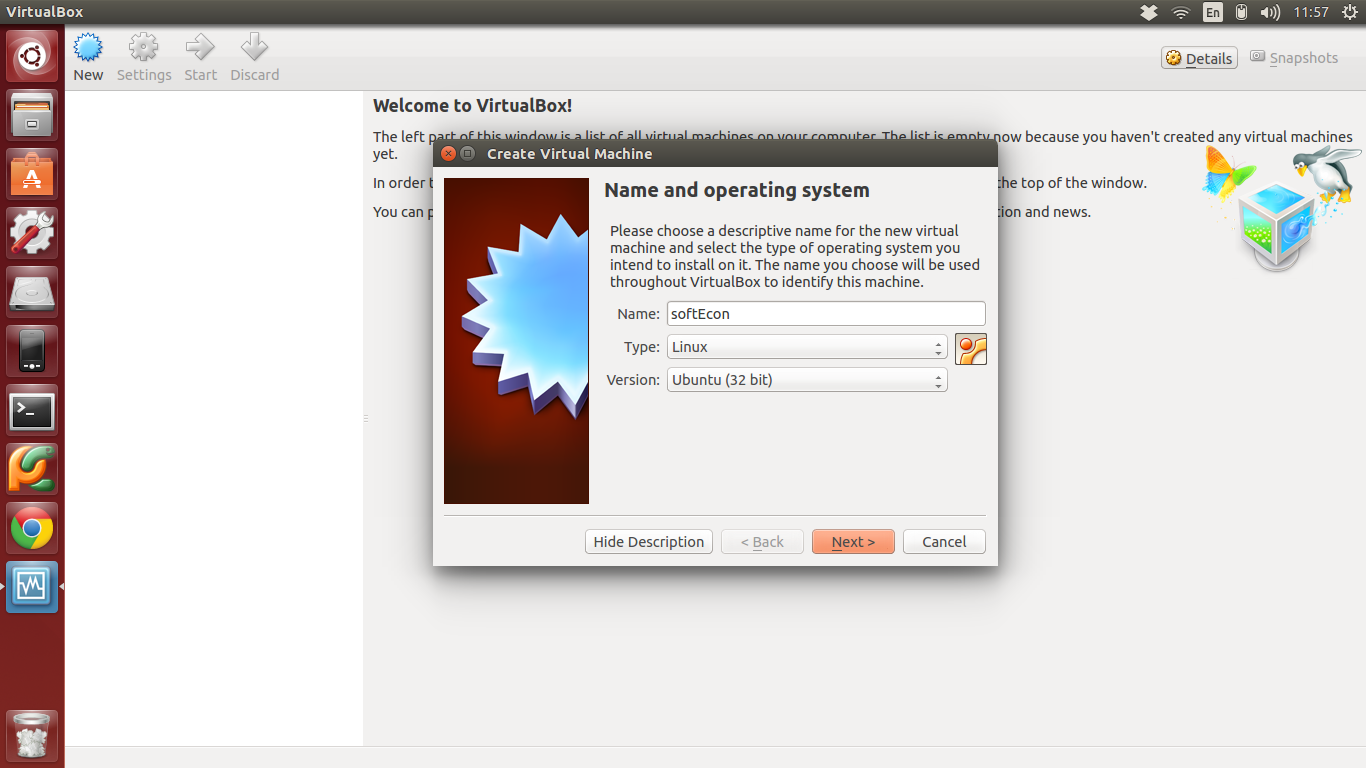
\includegraphics[width=0.8\textwidth]{material/virtualbox-start.png}
\end{figure}
%
The default settings work just fine and most can be modified later in the \textit{Vagrantfile}. We select a Virtual Machine Disk (VMDK) for the hard drive file type and assign 15GB (dynamically). The basic \textit{Ubuntu} installation already takes up around 7GB. \\\newline
%
When starting the virtual machine for the first time, we need to load the downloaded \textit{Ubuntu Desktop ISO} (Figure \ref{Startup Disk}).
%
\begin{figure}[h!]\centering\caption{Startup Disk}\vspace{0.3cm}\label{Startup Disk}
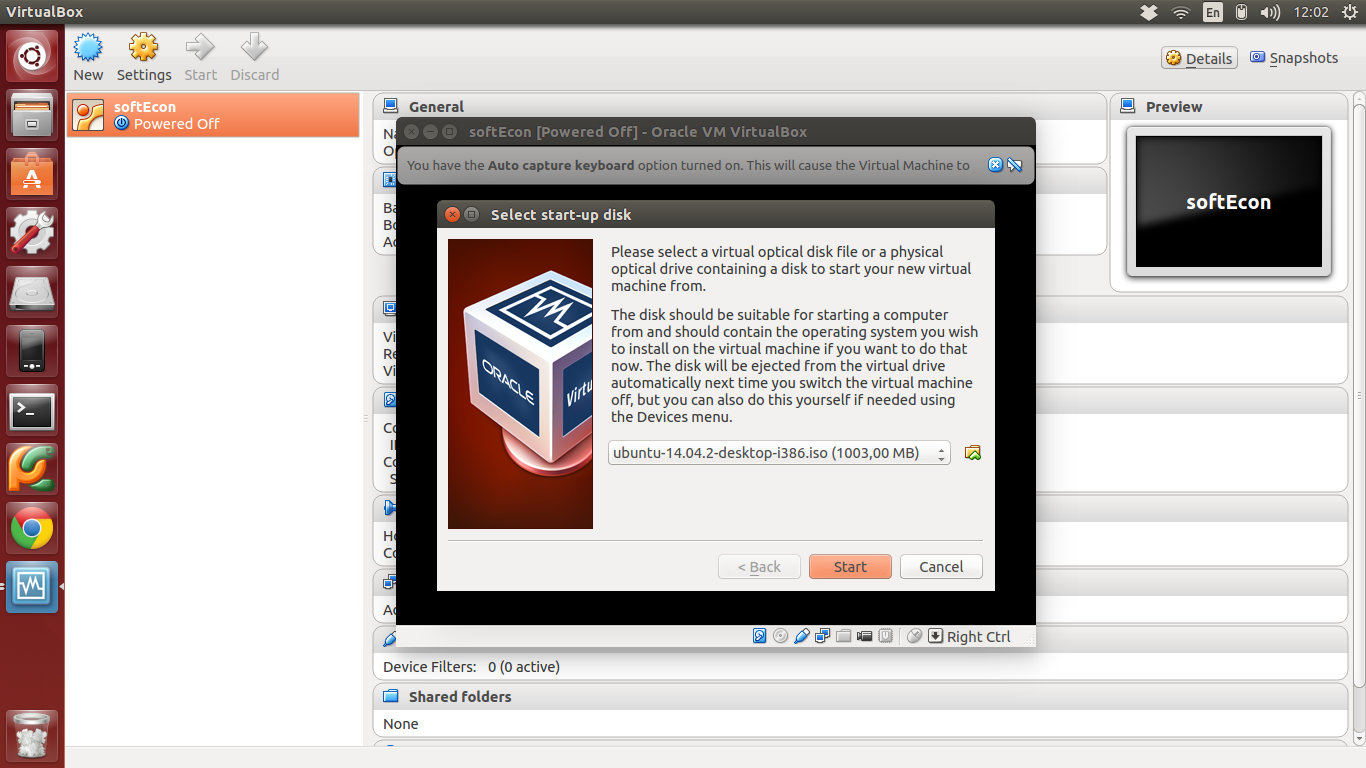
\includegraphics[width=0.8\textwidth]{material/startup-disk.png}
\end{figure}
%
This starts the usual \textit{Ubuntu} installation process. Again, the default settings work well. We just need to make sure to create a user \verb+vagrant+ and set its password to \verb+vagrant+. For the purpose of our class, we call the machine \verb+softEcon+ and will use this name for the rest of the instructions.  
%-------------------------------------------------------------------
\subsection*{Installing Guest Additions}
%-------------------------------------------------------------------
We will now install the \textit{VirtualBox Guest Additions}. These are a set of tools that provide closer integration between host and guest machine and improve the interactive performance of the guest system. Before installing the \textit{Guest Additions}, we have to extend the basic \textit{Ubuntu} installation to allow for building external kernel modules. We will make these installations using the terminal:
%
\vspace{0.2cm}\begin{lstlisting}[language=bash]
    $ sudo apt-get install dkms
    $ sudo apt-get install -y build-essential linux-headers-server
\end{lstlisting}\vspace{0.2cm}
%
We are ready to install the \textit{Guest Additions} by selecting the command in the \textit{Devices} tab inside \textit{VirtualBox}.
%-------------------------------------------------------------------
\subsection*{Preparing the VM}
%-------------------------------------------------------------------
Let us use the \textit{Software Updater} to get the latest updates installed. As we want to connect to the VM using secure shell (SSH) access, we will need to install the \textit{OpenSSH} server package as well. Then we shutdown the guest machine to ensure that all changes can take effect. Again, using the terminal:
%
\vspace{0.2cm}\begin{lstlisting}[language=bash]
    $ sudo apt-get update -y
    $ sudo apt-get install -y openssh-server
    $ sudo shutdown -r now
\end{lstlisting}\vspace{0.2cm}
%
We can restart the VM and now install additional software such as the \textit{SciPy Stack}:
%
\vspace{0.2cm}\begin{lstlisting}[language=bash]
    $ sudo apt-get install python-numpy python-scipy python-matplotlib 
    $ sudo apt-get install ipython ipython-notebook python-pandas 
    $ sudo apt-get install python-sympy python-nose
\end{lstlisting}\vspace{0.2cm}
%
Many aspects of \textit{Vagrant} expect the default SSH user to have passwordless \verb+sudo+ configured. This lets  \textit{Vagrant} configure networks, mount synced folders, install software, and more. We can set this up as follows:
%
\vspace{0.2cm}\begin{lstlisting}[language=bash]
    # Start interactive session with root privileges
    $ sudo -i
    # Edit the sudoers file
    $ visudo
\end{lstlisting}\vspace{0.2cm}
%
and append the following line to the file:
%
\vspace{0.2cm}\begin{lstlisting}[language=bash]
    vagrant ALL=(ALL) NOPASSWD:ALL
\end{lstlisting}\vspace{0.2cm}
%
After returning to the terminal, we now turn to the SSH access. By default,  \textit{Vagrant} expects a \verb+vagrant+ user to SSH into the machine. This user should be set up with the insecure keypair that  \textit{Vagrant} uses as a default to attempt to SSH. We can set this up:
%
\vspace{0.2cm}\begin{lstlisting}[language=bash]
    # Deposit the key
    $ mkdir -p /home/vagrant/.ssh
    $ wget --no-check-certificate \
    	https://raw.github.com/mitchellh/vagrant/master/keys/vagrant.pub \
    	-O /home/vagrant/.ssh/authorized_keys
    # Ensure correct permissions
    $ chmod 0700 /home/vagrant/.ssh
    $ chmod 0600 /home/vagrant/.ssh/authorized_keys
    $ chown -R vagrant /home/vagrant/.ssh
\end{lstlisting}\vspace{0.2cm}
%
We can reduce the size of the packaged box by running the following commands:
%
\vspace{0.2cm}\begin{lstlisting}[language=bash]
    # Write zeros to all empty spaces on the volume
    $ sudo dd if=/dev/zero of=/EMPTY bs=1M
    $ sudo rm -f /EMPTY
    # Shutdown the machine
    $ sudo shutdown -h now
\end{lstlisting}\vspace{0.2cm}
%
This shuts down the VM and concludes the setup of the machine. 
%-------------------------------------------------------------------
\section{Packaging and Testing the VM}
%-------------------------------------------------------------------
We are ready to create a \textit{Vagrant} base box on the host machine. It is important to turn to the packaging of the box directly and to not restart the VM at this point. Otherwise, the insecure keypair for SSH access is overwritten and the packaged box cannot be directly accessed by future users.
%
The following command creates a file \verb+package.box+.
%
\vspace{0.2cm}\begin{lstlisting}[language=bash]
    $ vagrant package --base softEcon
\end{lstlisting}\vspace{0.2cm}
%
We can test the SSH and GUI access by initializing a basic \textit{Vagrantfile} and specifying the use of the \verb+package.box+ for the startup.
%
\vspace{0.2cm}\begin{lstlisting}[language=bash]
    $ vagrant init package.box
\end{lstlisting}\vspace{0.2cm}
%
Let us test the SSH access:
\vspace{0.2cm}\begin{lstlisting} 
    $ vagrant up
    $ vagrant ssh
\end{lstlisting}\vspace{0.2cm}
%
If that works well, all that is left to check is the Graphical User Interface (GUI). We can activate it by uncommenting the following lines in the \textit{Vagrantfile}.
%
\vspace{0.2cm}\begin{lstlisting} 
    config.vm.provider "virtualbox" do |v|
        v.gui = true
    end
\end{lstlisting}\vspace{0.2cm}
%
These edits take effect once we reload our VM:
%
\vspace{0.2cm}\begin{lstlisting} 
    $ vagrant up reload
\end{lstlisting}
%-------------------------------------------------------------------
\section{Distributing the VM}
%-------------------------------------------------------------------
We use \textit{Atlas} at
%
\begin{center}
\url{https://atlas.hashicorp.com/softEcon/boxes/base}
\end{center}
% 
to distribute our box as this is the default hosting service (Figure \ref{Hashicorp}).
%
\begin{figure}[h!]\centering\caption{\textit{Vagrant} Cloud}\vspace{0.3cm}\label{Hashicorp}
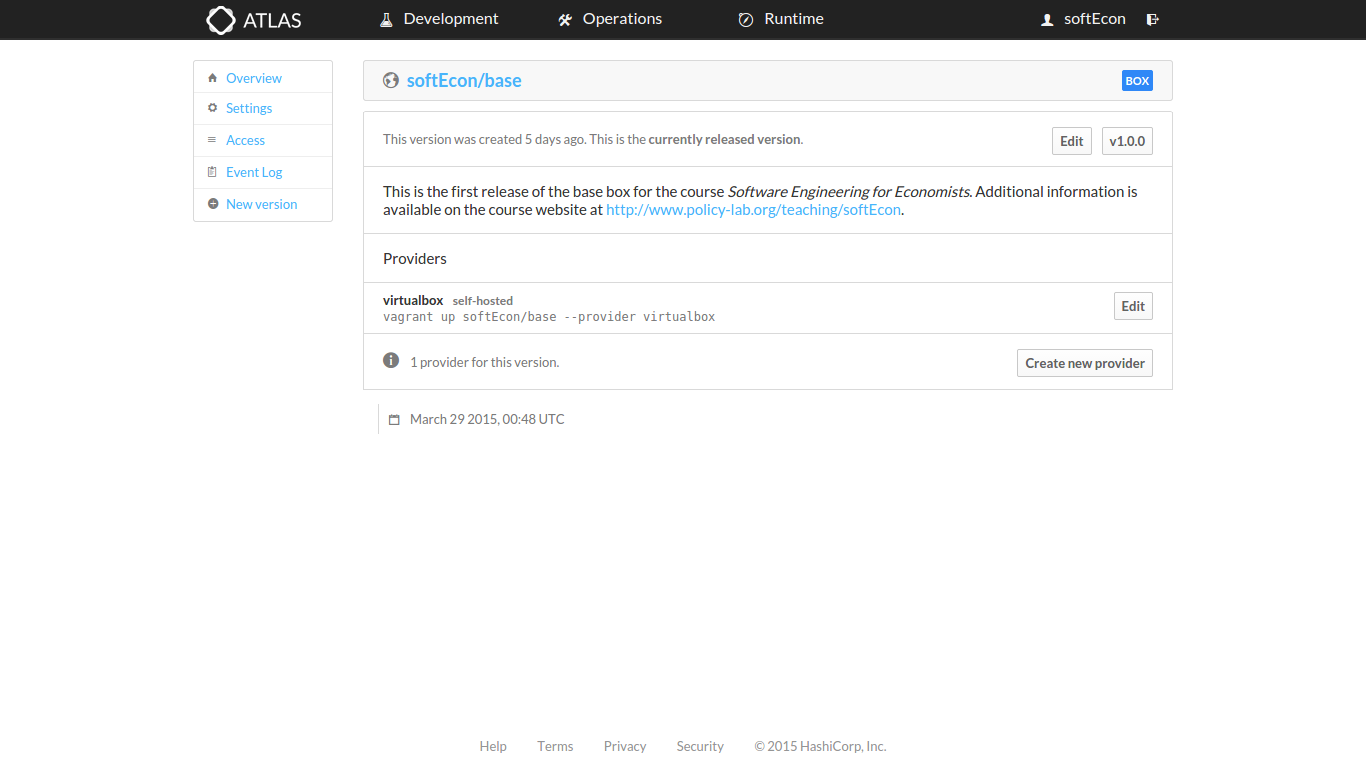
\includegraphics[width=0.8\textwidth]{material/hashicorp.png}
\end{figure}
%
After installing \textit{VirtualBox} and \textit{Vagrant}, students can start working on the VM simply by calling:
%
\vspace{0.2cm}\begin{lstlisting} 
$ vagrant init softEcon/base
$ vagrant up
$ vagrant ssh
\end{lstlisting}\vspace{0.2cm}
%
\noindent If you have any further questions or comments, please do not hesitate to let us know at \href{mailto:softEcon@policy-lab.org}{softEcon@policy-lab.org}.

\nocite{Hashimoto.2013}
\bibliography{../../../ext/bib/literature}
\bibliographystyle{apalike}

\end{document}
